% Options for packages loaded elsewhere
\PassOptionsToPackage{unicode}{hyperref}
\PassOptionsToPackage{hyphens}{url}
%
\documentclass[
]{article}
\usepackage{amsmath,amssymb}
\usepackage{iftex}
\ifPDFTeX
  \usepackage[T1]{fontenc}
  \usepackage[utf8]{inputenc}
  \usepackage{textcomp} % provide euro and other symbols
\else % if luatex or xetex
  \usepackage{unicode-math} % this also loads fontspec
  \defaultfontfeatures{Scale=MatchLowercase}
  \defaultfontfeatures[\rmfamily]{Ligatures=TeX,Scale=1}
\fi
\usepackage{lmodern}
\ifPDFTeX\else
  % xetex/luatex font selection
\fi
% Use upquote if available, for straight quotes in verbatim environments
\IfFileExists{upquote.sty}{\usepackage{upquote}}{}
\IfFileExists{microtype.sty}{% use microtype if available
  \usepackage[]{microtype}
  \UseMicrotypeSet[protrusion]{basicmath} % disable protrusion for tt fonts
}{}
\makeatletter
\@ifundefined{KOMAClassName}{% if non-KOMA class
  \IfFileExists{parskip.sty}{%
    \usepackage{parskip}
  }{% else
    \setlength{\parindent}{0pt}
    \setlength{\parskip}{6pt plus 2pt minus 1pt}}
}{% if KOMA class
  \KOMAoptions{parskip=half}}
\makeatother
\usepackage{xcolor}
\usepackage[margin=1in]{geometry}
\usepackage{longtable,booktabs,array}
\usepackage{calc} % for calculating minipage widths
% Correct order of tables after \paragraph or \subparagraph
\usepackage{etoolbox}
\makeatletter
\patchcmd\longtable{\par}{\if@noskipsec\mbox{}\fi\par}{}{}
\makeatother
% Allow footnotes in longtable head/foot
\IfFileExists{footnotehyper.sty}{\usepackage{footnotehyper}}{\usepackage{footnote}}
\makesavenoteenv{longtable}
\usepackage{graphicx}
\makeatletter
\def\maxwidth{\ifdim\Gin@nat@width>\linewidth\linewidth\else\Gin@nat@width\fi}
\def\maxheight{\ifdim\Gin@nat@height>\textheight\textheight\else\Gin@nat@height\fi}
\makeatother
% Scale images if necessary, so that they will not overflow the page
% margins by default, and it is still possible to overwrite the defaults
% using explicit options in \includegraphics[width, height, ...]{}
\setkeys{Gin}{width=\maxwidth,height=\maxheight,keepaspectratio}
% Set default figure placement to htbp
\makeatletter
\def\fps@figure{htbp}
\makeatother
\setlength{\emergencystretch}{3em} % prevent overfull lines
\providecommand{\tightlist}{%
  \setlength{\itemsep}{0pt}\setlength{\parskip}{0pt}}
\setcounter{secnumdepth}{5}
   \usepackage{xcolor}
   \usepackage{threeparttablex}
   \usepackage{longtable}
   \usepackage{subfig}
   \usepackage{mathptmx}
   \usepackage{unicode-math}
%\setmainfont{Latin Modern Roman} 
%\setmathfont{STIXTwoMath-Regular}
   \usepackage[scaled=1.1]{helvet}
   \renewcommand{\familydefault}{\rmdefault}
   

\newcommand{\bibfont}{\footnotesize}

%   \usepackage[authordate, backend=bibtex,sorting=nyt, natbib, ]{biblatex-chicago}
%   \usepackage[authordate]{biblatex-chicago}
%\DeclareFieldFormat[article]{title}{\mkbibquote{#1}} % make article titles in quotes
% \DeclareFieldFormat[thesis]{title}{\mkbibemph{#1}} % make theses italics

   \renewcommand{\bibfont}{\small}
   \usepackage{babel}
   \usepackage{fancyhdr}
   \usepackage{setspace}
   \usepackage{caption}
   \pagestyle{fancy}
   \usepackage{siunitx}
   \usepackage[capposition=top]{floatrow}
   \usepackage{dsfont}
   \usepackage{placeins}
   \usepackage{todonotes}
\usepackage[subfigure]{tocloft}
\usepackage{pgffor}
   \usepackage{csquotes}
   \usepackage[toc,page,title,titletoc,header]{appendix}    
   \usepackage{amsthm} % to introduce theorems etc.
   \usepackage{bm}
   \usepackage{bbm}  % Define \bm{} to use bold math fonts
   \usepackage{amssymb}
   \newtheorem{Theorem}{Theorem}
   \newtheorem{fact}{Fact}
   \newtheorem{mydef}{Definition}
   \usepackage[hang]{footmisc}	% Footnote formatting
   \renewcommand{\hangfootparindent}{1em}
   \renewcommand{\hangfootparskip}{0em}
   \renewcommand{\footnotemargin}{0.00001pt}
   \def\footnotelayout{\hspace{1em}}%
   \def\footnotelayout{\hspace{1em}}%
   \renewcommand\thepart{\hspace{1cm} \arabic{part}}
   \renewcommand\thesection{\Roman{section}}
   \renewcommand\thesubsection{\thesection.\arabic{subsection}}
   \renewcommand\thesubsubsection{\Alph{subsubsection}}
   \renewcommand\theparagraph{\alph{paragraph})}
   \renewcommand\thesubparagraph{\roman{subparagraph})}
   \usepackage[nobottomtitles*]{titlesec}
   \titleformat{\chapter}[display]{\normalfont\huge\bfseries}{\chaptertitlename\ \thechapter.}{20pt}{\Huge}
   \titleformat{\section}{\normalfont\Large\bfseries}{\thesection}{1em}{}
   \titleformat{\subsection}{\normalfont\large\bfseries}{\thesubsection}{1em}{}
   \titleformat{\subsubsection}{\normalfont\normalsize\bfseries}{\thesubsubsection)}{1em}{}
   \titleformat{\paragraph}[runin]{\normalfont\normalsize\bfseries}{\theparagraph}{1em}{}
   \titleformat{\subparagraph}[runin]{\normalfont\normalsize\bfseries}{\thesubparagraph}{1em}{}
   \titlespacing*{\chapter} {0pt}{50pt}{40pt}
   \titlespacing*{\section} {12pt}{3.5ex plus 1ex minus .2ex}{2.3ex plus .2ex}
   \titlespacing*{\subsection} {24pt}{3.25ex plus 1ex minus .2ex}{1.5ex plus .2ex}
   \titlespacing*{\subsubsection}{36pt}{3.25ex plus 1ex minus .2ex}{1.5ex plus .2ex}
   \titlespacing*{\paragraph} {0pt}{3.25ex plus 1ex minus .2ex}{1em}
   \titlespacing*{\subparagraph} {24pt}{3.25ex plus 1ex minus .2ex}{1em}
   

   
   \newcommand{\esp}[1]{\mathds{E}[ #1 ]}
   \newcommand{\espb}[1]{\mathds{E}\Big[ #1 \Big]}
   \newcommand{\var}[1]{\mathds{V}[ #1 ]}
   \newcommand{\one}[1]{\mathds{1}( #1 )}
   \newcommand{\normal}[1]{\mathcal{N}}
   \usepackage{etoolbox} %— available from CTAN (required)–
   \usepackage{keyval}%— a standard package (required)–
   \usepackage{ifthen}%— a standard package (required)–
   \usepackage{graphicx} % You need this for the headers
   \definecolor{ForestGreen}{RGB}{34,139,34}
   \usepackage{booktabs}
    \newcolumntype{d}{S[
      input-open-uncertainty=,
      input-close-uncertainty=,
      parse-numbers = false,
      table-align-text-pre=false,
      table-align-text-post=false
       ]}
    \usepackage{algorithm}
    %\usepackage{algorithm2e}
    \usepackage{algpseudocode}
     \usepackage{pgfgantt}
     \usepackage{tikz}
     \usetikzlibrary{arrows.meta}
      \usetikzlibrary{arrows}
      \usetikzlibrary{patterns}
      \usepackage{fontspec}
      \setmainfont{Times New Roman}
      \renewcommand\qedsymbol{\emph{QED}}
      \newcommand\blfootnote[1]{%
      \begingroup
      \renewcommand\thefootnote{}\footnote{#1}%
      \addtocounter{footnote}{-1}%
      \endgroup}
      
% add more space for table and figure to avoid floating
\renewcommand{\topfraction}{.85}
\renewcommand{\bottomfraction}{.7}
\renewcommand{\textfraction}{.15}
\renewcommand{\floatpagefraction}{.66}
\setcounter{topnumber}{3}
\setcounter{bottomnumber}{3}
\setcounter{totalnumber}{4}

%\AtBeginDocument{\let\maketitle\relax}      
\usepackage{flafter}
\usepackage{float}
\usepackage{tabularray}
\usepackage[normalem]{ulem}
\usepackage{graphicx}
\UseTblrLibrary{booktabs}
\UseTblrLibrary{rotating}
\UseTblrLibrary{siunitx}
\NewTableCommand{\tinytableDefineColor}[3]{\definecolor{#1}{#2}{#3}}
\newcommand{\tinytableTabularrayUnderline}[1]{\underline{#1}}
\newcommand{\tinytableTabularrayStrikeout}[1]{\sout{#1}}
\ifLuaTeX
  \usepackage{selnolig}  % disable illegal ligatures
\fi
\usepackage[]{natbib}
\bibliographystyle{plainnat}
\usepackage{bookmark}
\IfFileExists{xurl.sty}{\usepackage{xurl}}{} % add URL line breaks if available
\urlstyle{same}
\hypersetup{
  pdftitle={Formal stuff POSAJE},
  pdfauthor={Arthur Heim},
  hidelinks,
  pdfcreator={LaTeX via pandoc}}

\title{Formal stuff POSAJE}
\author{Arthur Heim}
\date{2025-01-31}

\begin{document}
\maketitle

We model the decision to apply for childcare as a function of perceived eligibility, transaction costs, and potential benefits. Households face uncertainty regarding their eligibility and the costs associated with the application process. The intervention aims to reduce these frictions through information provision and administrative support.

We consider a sequential decision process where at the first period (baseline),
a pregnant woman has \emph{ex-ante} unobserved \textbf{preference profile} \(\theta_0\) with regard to future childcare options. We observe a set of observable attributes \(\mathbf{X}\) and intention to use \(I_0\). Among X, there are social group metrics (\(G\)) such as SES status (based on education), migration background, and rough metrics of temporal preferences \(\rho\) and knowledge of childcare \(\mathcal{I}\). There are also cognitive and structural factor that may hinder decisions. Let \(\mathcal{C}\) denote the subjective application costs.

In the absence of intervention, the decision to apply can define a latent propensity to apply:

\begin{equation}
I_0^*=\mu_w(\mathbf{Z})-U_I(\mathcal{I},\theta,\mathcal{C}),\quad I_0=1 ~ if ~I^*\geq 0,\quad I_0=0~otherwise
\end{equation}

Where \(\mathbf{Z}\) is a set of observables and \(U_I\) is unobserved and depend on information sets, preference types and subjective costs of application. We assume that \(\mathbf{Z}\perp U_I\)

\subsection{Intention gap by social groups}\label{intention-gap-by-social-groups}

Formally, the gap between two sets of values of covariates \(\mathbf{x}\) \(\mathbf{x^\prime}\) in intention to use at baseline is:

\begin{equation}
\Delta_{x,x'}(I_{0}) = \espb{I_{0i}|\mathbf{X}=\mathbf{x}}-\espb{I_{0i}|\mathbf{X}=\mathbf{x^\prime}}
\end{equation}

With a random sample, these conditional differences in reported intention to use childcare can be estimated using OLS and heteroskedasticity robust standard errors (Linear probability model) or by first estimating a model with parametric restrictions on \(I_0^*\) (such as logit or probit) and computing marginal effects.

However, these parameters and sample analogues are only descriptive difference in means between two groups who also differs in observable characteristics and latent \(U_I\).

We assume that the sampling process of our baseline sample is randomly drawn from the superpopulation
These difference in probabiliry

Idée générale :
Present oriented --\textgreater{} future benefits and costs
Utility of with or without childcare - cost of childcare + subjective costs

How reducing friction costs may affect different people (choice function)

\subsection{Adaptation of Castell et al.~(2024)}\label{adaptation-of-castell-et-al.-2024}

Pregnant woman must decide in the future whether they want childcare. Let b be the probability of receiving childcare (i.e.~successful application).
Application is an action \(A \in \{0,1\}\) equals to 1 if the access probability perceived with some error \(\epsilon\) exceeds application costs \(c\).

\begin{equation}
A =\one{b+\epsilon-c>0}
\end{equation}

A mother may not apply if she lack information or underestimate her chance of access (\epsilon\textless0), she may face transaction costs \(c\) which are non-monetary costs going through application process such as complexity, delays, and so on.

\subsubsection{Information}\label{information}

Each individual is characterized by the value of the cost \(c\) and the error \(ε\) they make in the perception of the probability of access. We denote with \(F (x) = P (b < x)\) the cumulative distribution function of benefits b given \(c\) and \(\epsilon\). The probability to apply is:

\begin{equation}
P(A=1) =P(b>c-\epsilon)=1-F(c-\epsilon)
\end{equation}

Providing full information on application likelihood has the following effect on application:

\begin{equation}
\Delta(c,\epsilon)=P(b>c)-P(b>c-\epsilon)=F(c-\epsilon)-F(c)
\end{equation}

The effect of the information treatment is thus positive for agents who underestimate their access probability \((\epsilon < 0)\) and negative otherwise. The ITT effect sums \(\Delta(c,\epsilon)\) over the joint distribution of \((c,\epsilon)\).

Therefore, providing information increases application if, under imperfect information, there are more individuals who would benefit from applying but do not apply because they underestimate their eligibility than individuals whose net benefit is negative but who apply because they overestimate their eligibility.

Given our empirical results, it is useful to consider the reasons for why providing information may have no or very small effects on applications. First, it could be that on average agents have accurate beliefs, even though many of them are wrong about their own eligibility. Second, it could be that the effect of erroneous beliefs is small as compared to that of transaction costs, such that for most people with \(F (c − \epsilon) = 1\) (no take-up), we also have \(F (c) = 1\). Finally, it could simply be that \(\epsilon\) is uniformly zero, i.e.~that there are no information frictions.

\subsection{Administrative support}\label{administrative-support}

Application costs. We next investigate the impact of reducing application costs. We define \(c_0\), as the application cost one faces when supported by a caseworker, i.e.~when one receives treatment T2.

On their own (untreated), agents face a larger cost \(c \in\left[c_0, \infty\left[\right.\right.\) that is distributed in the population. Given our empirical results, let us consider a situation where imperfect information can be neglected \((\varepsilon=0)\). Then, the effect of this treatment for any agent of type \(c\) is:

\[
\Delta(c)=P\left(b>c_0\right)-P(b>c)=F(c)-F\left(c_0\right) \geq 0
\]

The population effect sums \(\Delta(c)\) over the marginal distribution of \(c\), and is positive. Note that in this case, the probability to apply and the probability to access are identical; the latter is more easily observable. The effect is stronger on agents that face higher transaction costs in the absence of treatment:

\[
\frac{\partial \Delta(c)}{\partial c}=f(c)>0
\]

To understand the effect of application costs on access, we also consider the treatment effect on access by the average claimant:

\[
\Delta^b(c)=E\left(b \mid b>c_0\right)-E(b \mid b>c)=\frac{\int_{c_0}^{\infty} b f(b) d b}{1-F\left(c_0\right)}-\frac{\int_c^{\infty} b f(b) d b}{1-F(c)}
\]

For any agent of type \(c\) this quantity is negative if \(c>c_0\) and zero otherwise. Integrating over \(c\) yields:

\[
\Delta^b=\int_0^{\infty} \Delta^b(c) g(c) d c
\]

If b and c are uncorrelated in the population, then \(\Delta^b\) is negative: lowering application costs extends access to people with lower claims. This corresponds to the idea that application costs are ordeals mechanisms that improve targeting (Kleven and Kopczuk, 2011; Alatas et al., 2016). If b and c are sufficiently positively correlated however, i.e.~if those most likely to get access also have higher costs, then \(\Delta^b\) can be positive. In that case lowering application costs can attract more parents who are more likely to access childcare (Deshpande and Li, 2019; Gupta, 2017).

\subsection{Compliance}\label{compliance}

In practice, the intervention is a phone call to which potentially eligible people may not answer or refuse the administrative support. In addition to the decision to apply to childcare, we need to model the decision to comply with the administrative support treatment as we can only identify treatment impact on compliers. Let us assume that mothers decide to take support by comparing the anticipated reduced cost of application \(\left(b-c_0\right)\) with nuisance from the intervention which we denote with \(\kappa>0\). An agent complies with the invitation if:

\[
b>c_0+\kappa
\]

In our analysis, we are interested not only in the average treatment effect, but also in the shape of the marginal treatment effect as a function of the cost of participation \(\kappa\), following Heckman (2010). We define the marginal treatment effect (MTE) as the effect of the treatment on the compliers, conditional on a value of the cost of administrative support, \(\kappa\), for any individual with application cost \(c\). The MTE is:

\[
\begin{aligned}
\operatorname{MTE}(\kappa ; c) & =P\left(b>c_0 \mid b>c_0+\kappa ; c\right)-P\left(b>c \mid b>c_0+\kappa ; c\right) \\
& =1-\frac{1-F(c)}{1-F\left(c_0+\kappa\right)}
\end{aligned}
\]

if \(\kappa<c-c_0\) and zero otherwise. Conditional on \(c\), we have:

\[
\frac{\partial M T E(\kappa ; c)}{\partial \kappa} \leq 0
\]

As \(\kappa\) grows, compliers are more and more selected towards higher chance of access \(b\); they find value in attending the meeting because it reduces their administrative burden, but the share that would apply even in the absence of the treatment grows, so that the treatment effect decreases. This is true for a given \(c\). We take the integral over \(c\) to obtain the MTE for the whole population:

\[
\operatorname{MTE}(\kappa)=\int_{c_0}^{\infty} M T E(\kappa ; c) g(c \mid \kappa) d c
\]

When \(\kappa\) increases, every \(\operatorname{MTE}(\kappa ; c)\) in the integral decreases. If \(c\) and \(\kappa\) are uncorrelated, then \(\operatorname{MTE}(\kappa)\) will also be a decreasing function of \(\kappa\). But if \(c\) and \(\kappa\) are positively correlated, the MTE can be increasing in \(\kappa\), since the large \(\operatorname{MTE}(\kappa ; c)\) with large \(c\) receive a higher weight \(g(c \mid \kappa)\). Claimants who face large transaction costs and would benefit the most from administrative support also face large costs of accepting it.

\section{Setting}\label{setting}

\subsection{Baseline}\label{baseline}

Pregnant woman \(i\) at time \(t_0\) have a set of observable attributes bundled in a matrix \(\mathbf{A}_0\) and an unobservable set of information \(\mathcal{I}\). In addition, Let \(\mathbf{X} \subset \mathbf{A}\) denote fixed attributes
(e.g.~measures of social groups) and let \(\mathbf{K}\subset \mathbf{A}\backslash X\) some observed metrics for preferences, knowledge, norms, values, and so on.
In particular, we observe women intention to use childcare and their most favourite childcare arrangement.

\(\mathbf{X}\) and \(\mathbf{K}\) may be correlated as unobserved factor determine both observed characteristics such as social groups and preferences, norms, intention to use childcare\ldots{}

\subsubsection{Ex-ante preference profiles}\label{ex-ante-preference-profiles}

Woman must choose whether she applies to formal childcare and more precisely which childcare types.
Assume for simplicity that the choice set is sparse such that she can choose to apply to Daycare \(D\), Childminder \(C\) and if she doesn't apply to one of the two, the default is parental care \(P\).
Woman \(i\) has \(ex-ante\) preference order over childcare solutions we denote \(\succeq_i\) which can be:

\begin{equation}
    \succ_i \equiv 
      \left\{ 
          \begin{aligned}
            \left. 
              \begin{matrix}
                a:=D\succeq_iC\succeq_iP    \\
                b:=C\succeq_iD\succeq_iP    \\
              \end{matrix} 
            \} \right. & 
                \text{childcare enthusiasts} ~~;    \\
            \left. 
              \begin{matrix}
                c:=D\succeq_iP\succeq_iC\\
                d:=C\succeq_iP\succeq_iD\\
              \end{matrix}
            \} \right. & 
                  \text{Selective parents} ~~;    \\
            \left. 
              \begin{matrix}
                e:=P\succeq_iC\succeq_iD\\
                f:=P\succeq_iD\succeq_iC\\
              \end{matrix} 
            \}\right. & 
                  \text{Parental care } ~~;  \\
          \end{aligned} 
    \right.
\end{equation}

We can also bundle preference profiles by ``daycare enthusiasts'', ``childminder enthusiasts''.

\begin{equation}
    \succ_i \equiv 
      \left\{ 
          \begin{aligned}
            \left. 
              \begin{matrix}
                a:=D\succeq_iC\succeq_iP    \\
                c:=D\succeq_iP\succeq_iC\\
              \end{matrix} 
            \} \right. & 
                \text{Daycare enthusiasts} ~~;    \\
            \left. 
              \begin{matrix}
                d:=C\succeq_iP\succeq_iD\\
                b:=C\succeq_iD\succeq_iP    \\
              \end{matrix}
            \} \right. & 
                  \text{Childminder enthusiasts} ~~;    \\
            \left. 
              \begin{matrix}
                e:=P\succeq_iC\succeq_iD\\
                f:=P\succeq_iD\succeq_iC\\
              \end{matrix} 
            \}\right. & 
                  \text{Parental care} ~~;  \\
          \end{aligned} 
    \right.
\end{equation}

At \(t_0\), childcare enthusiasts and selective parents reveal their intention to use and most preferred childcare. therefore, we observe the following preference types in the data. Let \(W\) denote intention to use.

\begin{itemize}
\tightlist
\item
  those who intend to use childcare and prefer daycare have preference types \(\succeq_i\in\{a,c\}\) : the daycare enthusiasts
\item
  those who intend to use childcare and prefer childminders have preference types \(\succeq_i\in\{b,d\}\): the childminder enthusiasts
\item
  Those who do not intend to use childcare have preference types \(\succeq_i\in\{e,f\}\): those who would rather care for their children themselves.
\end{itemize}

If we knew if the parent would accept another childcare and assume strict preference order, we could classify parents of all 6 preference types at baseline. But we don't. Therefore, these types are unknown.

Moreover, these preference types evolve over time as parents' situation, information sets, needs etc. change.
There are also cognitive and structural factor that may hinder decisions. Let \(\mathcal{C}\) denote the subjective application costs.

In the absence of intervention, the decision to apply can define a latent propensity to apply:

\begin{equation}
W^*(0)=\mu_w(\mathbf{Z})-U_w(\mathcal{I},\succeq,\mathcal{C}),\quad W=1 ~ if ~W^*\geq 0,\quad W=0~otherwise
\end{equation}

Where \(\mathbf{Z}\) is a set of observables and \(U_w\) is unobserved and depend on information sets, preference types and subjective costs of application.

\subsection{Endline data}\label{endline-data}

The endline survey includes the different sets of outcomes including some metrics of knowledges, application behaviours and access to formal childcare. We leave attrition issues for now and focus on application behaviours. We come back to these points later.

Let \(\tilde{Y_i}=\one{\text{applied to any childcare}}\) be the endline measure of application behaviours which derive from:
\[
\tilde{Y}_{i}=\underbrace{\one{\text{applied for childminders}}}_{Y^c}+\underbrace{\one{\text{applied for daycare}}}_{Y^d}\\
\]
In practice, \(\tilde{Y}\) also include other childcare arrangement.

The relationships between the observed variables from Baseline and Endline can be represented using Directed Acyclic Graphs such as Figure \ref{fig:DagIntention}. This model is not identified. No causal relationship can be inferred.

\begin{figure}
\centering
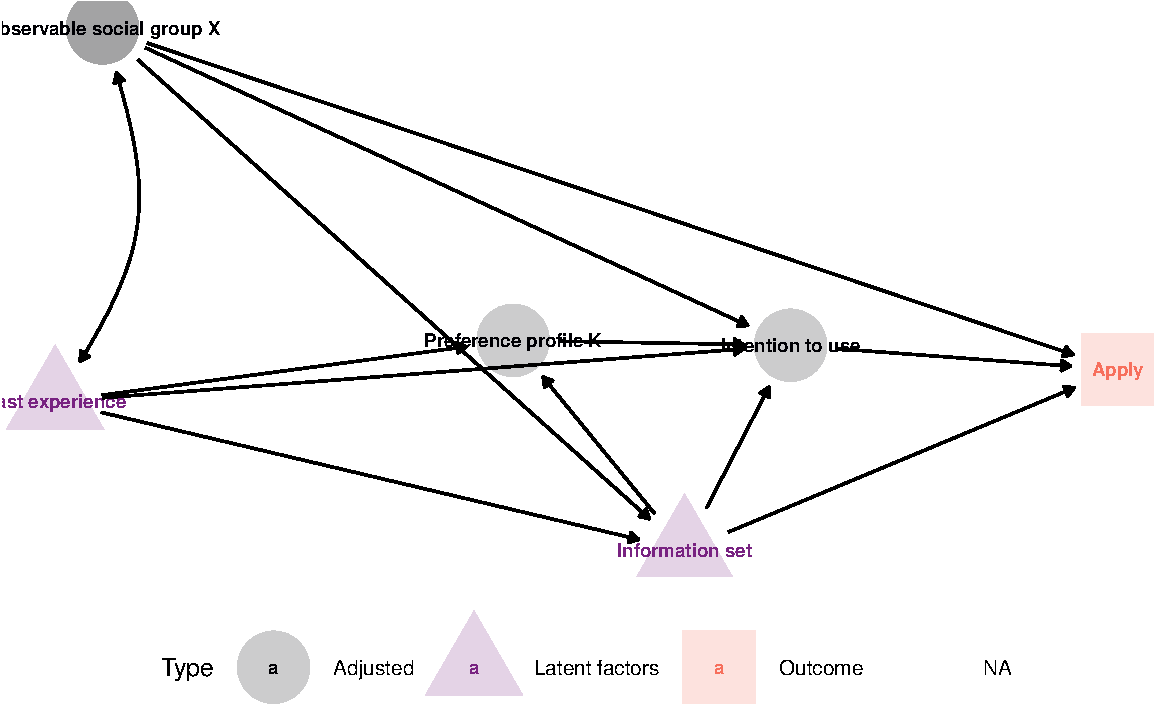
\includegraphics{FormalStuff_files/figure-latex/DagIntention-1.pdf}
\caption{\label{fig:DagIntention}How observed baseline characteristics relate with the main outcome.}
\end{figure}

\subsection{Intention to action gap}\label{intention-to-action-gap}

We analyse the intention-to-action gap between different social groups (High/low SES, migration background) (\(\mathbf{X}\)) and subjective attributes (Information, temporal orientation) (\(\mathbf{K}\)).

Formally, the gap between two sets of values of covariates \(\mathbf{x}\) \(\mathbf{x^\prime}\) in intention to use at baseline is:

\begin{equation}
\Delta_{x,x'}(W_i) = \espb{W_i|\mathbf{X}=\mathbf{x}}-\espb{W_i|\mathbf{X}=\mathbf{x^\prime}}
\end{equation}

The application gap is :

\begin{equation}
\Delta_{x,x'}(\tilde{Y}_i) = \espb{\tilde{Y}_i|\mathbf{X}=\mathbf{x}}-\espb{\tilde{Y}_i|\mathbf{X}=\mathbf{x^\prime}}
\end{equation}

Denoting \(\tilde{Y^*}\) the variable for access to formal childcare, The access gap is :

\begin{equation}
\Delta_{x,x'}(\tilde{Y*}_i) = \espb{\tilde{Y^*}_i|\mathbf{X}=\mathbf{x}}-\espb{\tilde{Y^*}_i|\mathbf{X}=\mathbf{x^\prime}}
\end{equation}

In our setting, the covariates are discrete. These three parameters can therefore be estimated from the control group by regressing the outcome on group dummies using OLS and heterokedasticity robust standard errors, or by computing marginal effects from a logit or probit model.
OLS estimates are reported in Figure \ref{fig:AttentionAction}.

\begin{figure}[H]
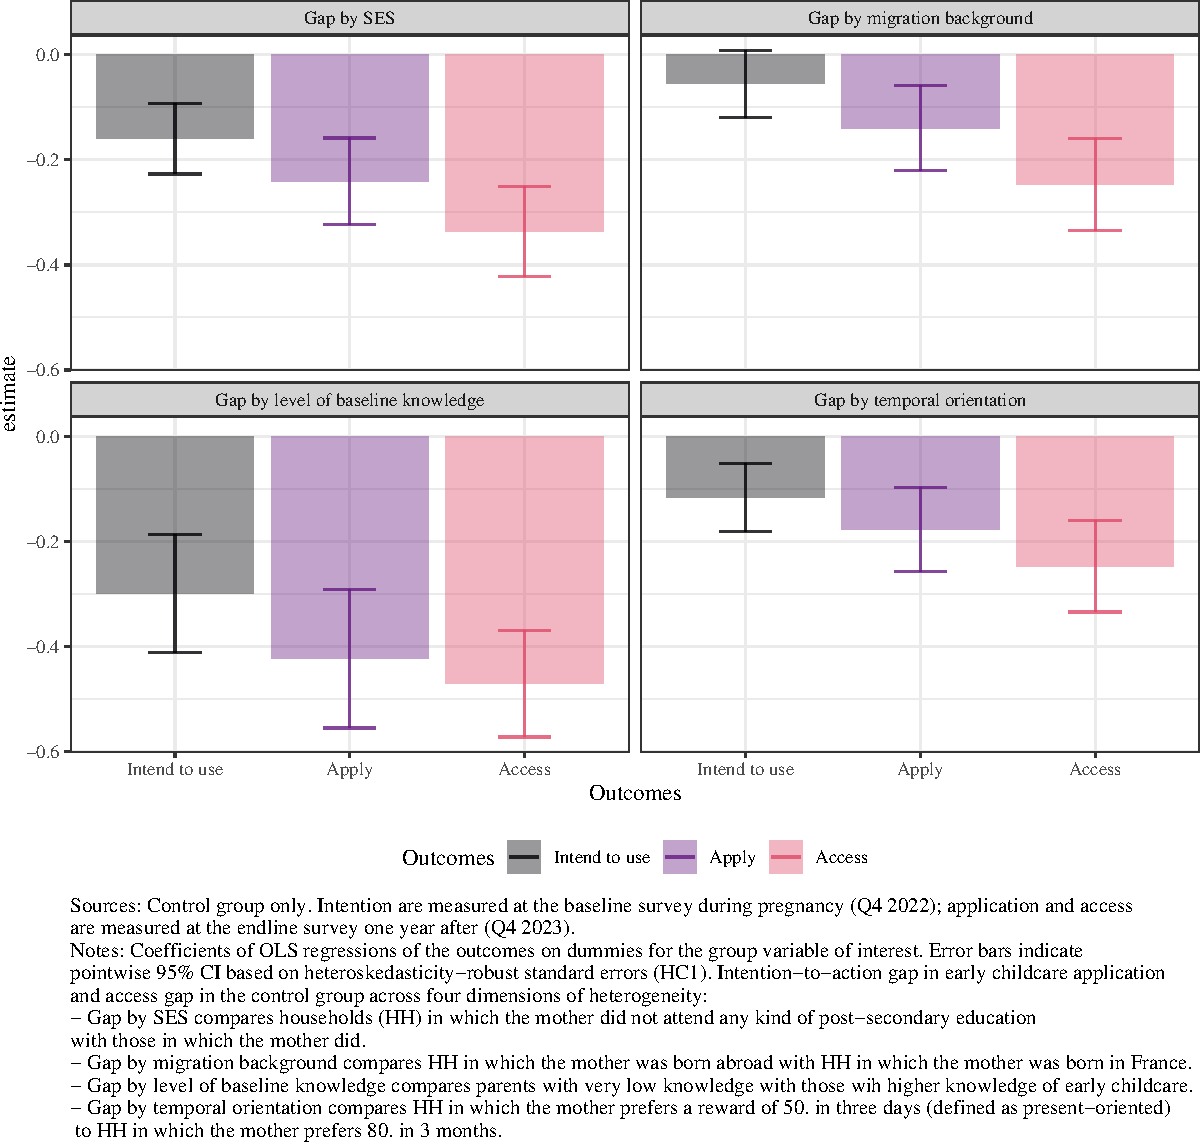
\includegraphics[width=1\linewidth]{FormalStuff_files/figure-latex/AttentionAction-1} \caption{ The intention-to-action gap in early childcare application and access in the control group across four dimensions of heterogeneity. Intention to use early childcare is measured at the baseline survey during pregnancy. Early childcare application and early childcare access are measured at the endline survey one year after.}\label{fig:AttentionAction}
\end{figure}

\begin{table}
\centering
\begin{tblr}[         %% tabularray outer open
]                     %% tabularray outer close
{                     %% tabularray inner open
colspec={Q[]Q[]Q[]Q[]},
column{2,3,4}={}{halign=c,},
column{1}={}{halign=l,},
hline{10}={1,2,3,4}{solid, black, 0.05em},
}                     %% tabularray inner close
\toprule
& Simple dif & Residualised MW & Fixed Effect \\ \midrule %% TinyTableHeader
(Intercept)               & \num{0.864}              & \num{0.000}              &                           \\
& (\num{0.018})            & (\num{0.016})            &                           \\
Educ2Low-SES              & \num{-0.160}             &                           &                           \\
& (\num{0.034})            &                           &                           \\
resEduc                   &                           & \num{-0.153}             &                           \\
&                           & (\num{0.035})            &                           \\
LowSES                    &                           &                           & \num{-0.153}             \\
&                           &                           & (\num{0.035})            \\
Num.Obs.                  & \num{623}                & \num{623}                & \num{623}                \\
R2                        & \num{0.038}              & \num{0.034}              & \num{0.041}              \\
R2 Adj.                   & \num{0.037}              & \num{0.032}              & \num{0.028}              \\
R2 Within                 &                           &                           & \num{0.034}              \\
R2 Within Adj.            &                           &                           & \num{0.032}              \\
AIC                       & \num{603.7}              & \num{602.1}              & \num{616.1}              \\
BIC                       & \num{612.5}              & \num{610.9}              & \num{656.0}              \\
RMSE                      & \num{0.39}               & \num{0.39}               & \num{0.39}               \\
Std.Errors                & Heteroskedasticity-robust & Heteroskedasticity-robust & Heteroskedasticity-robust \\
Mean of DV                & 0.80                      & -0.00                     & 0.80                      \\
FE: MaternityWardBaseline &                           &                           & X                         \\
\bottomrule
\end{tblr}
\end{table}

If one think that because sampling was done in different maternity wards which may be used by different mothers such that there are intra-maternity ward correlation of outcomes, inference should rely on cluster-robust standard errors adjusted at the maternity ward level. Controlling for maternity ward dummies would remove the correlation with the social group variable and the between maternity ward difference in outcomes (by the FWL theorem).

Another parameter of interest is the intention to action gap, and differences between social groups.
We can compute

\begin{enumerate}
\def\labelenumi{\arabic{enumi})}
\tightlist
\item
  the share of parents who applied by baseline intention
\item
  the shares of parents who applied by baseline intention and SES group
\end{enumerate}

\begin{table}
\centering
\begin{tblr}[         %% tabularray outer open
]                     %% tabularray outer close
{                     %% tabularray inner open
colspec={Q[]Q[]Q[]Q[]},
column{2,3,4}={}{halign=c,},
column{1}={}{halign=l,},
hline{22}={1,2,3,4}{solid, black, 0.05em},
}                     %% tabularray inner close
\toprule
& (1) & (2) & (3) \\ \midrule %% TinyTableHeader
factor(ECSPlanToBaseline)0                    & \num{0.295}              &                           &                           \\
& (\num{0.047})            &                           &                           \\
factor(ECSPlanToBaseline)1                    & \num{0.850}              &                           &                           \\
& (\num{0.018})            &                           &                           \\
ECSPlanToBaseline = 0 × Educ2 = High-SES      &                           & \num{0.375}              &                           \\
&                           & (\num{0.077})            &                           \\
ECSPlanToBaseline = 0 × Educ2 = Low-SES       &                           & \num{0.236}              &                           \\
&                           & (\num{0.058})            &                           \\
ECSPlanToBaseline = 1 × Educ2 = High-SES      &                           & \num{0.903}              &                           \\
&                           & (\num{0.018})            &                           \\
ECSPlanToBaseline = 1 × Educ2 = Low-SES       &                           & \num{0.742}              &                           \\
&                           & (\num{0.038})            &                           \\
i(Educ2, ECSPlanToBaseline, ref = "High-SES") &                           &                           & \num{-0.022}             \\
&                           &                           & (\num{0.105})            \\
ECSPlanToBaseline                             &                           &                           & \num{0.528}              \\
&                           &                           & (\num{0.079})            \\
Educ2High-SES                                 &                           &                           & \num{0.375}              \\
&                           &                           & (\num{0.077})            \\
Educ2Low-SES                                  &                           &                           & \num{0.236}              \\
&                           &                           & (\num{0.058})            \\
Num.Obs.                                      & \num{494}                & \num{494}                & \num{494}                \\
R2                                            & \num{0.249}              & \num{0.278}              & \num{0.278}              \\
R2 Adj.                                       & \num{0.247}              & \num{0.273}              & \num{0.273}              \\
AIC                                           & \num{445.7}              & \num{430.4}              & \num{430.4}              \\
BIC                                           & \num{454.1}              & \num{447.2}              & \num{447.2}              \\
RMSE                                          & \num{0.38}               & \num{0.37}               & \num{0.37}               \\
Std.Errors                                    & Heteroskedasticity-robust & Heteroskedasticity-robust & Heteroskedasticity-robust \\
Mean of DV                                    & 0.74                      & 0.74                      & 0.74                      \\
\bottomrule
\end{tblr}
\end{table}

The first one shows how many parents switch preference types by moving from intention to no application and vice versa.
There are 29\% who didn't want childcare but did apply ; and 85\% who intended to use but didn't apply.

The second column separate these averages by SES group. Interestingly, Low SES groups who did not intend to use are 24\% to apply while High SES groups are 38\% to switch.
However, 90\% High SES group who intended to use did apply while only 74\% of Low SES did.
High SES parents who already intended to apply are more likely to commit to this intention and those who didn't intend to use are more likely to have changed their mind.
On the contrary, Low-SES who intended to use daycare are less likely to commit to their choice and those who didn't intend to use are less likely to change their mind.

\begin{align}
\Delta_{x,x'}(\tilde{Y}_i-W_i) &=& \espb{\tilde{Y}_i-W_i|\mathbf{X}=\mathbf{x}}-\espb{\tilde{Y}_i-W_i|\mathbf{X}=\mathbf{x^\prime}}\\
&=&  \underbrace{\espb{\tilde{Y}_i|\mathbf{X}=\mathbf{x}}-\espb{\tilde{Y}_i|\mathbf{X}=\mathbf{x^\prime}}}_{\Delta_{x,x'}(\tilde{Y}_i)}-\underbrace{\left(\espb{W_i|\mathbf{X}=\mathbf{x}}-\espb{W_i|\mathbf{X}=\mathbf{x^\prime}}\right)}_{\Delta_{x,x'}(W_i)}
\end{align}

This parameter can be estimated either by regressing the difference between application and intention on social group dummies or by:

\begin{enumerate}
\def\labelenumi{\arabic{enumi})}
\tightlist
\item
  stacking baseline and endline databases
\item
  defining an outcome \(Y\) which equals \(W\) in the baseline and \(\tilde{Y}\) in the endline.
\item
  regressing Y on an endline dummy, an interaction with the group indicator and mother fixed effects and clustered SE
\end{enumerate}

The coefficient of the interaction is an estimate of \(\Delta_{x,x'}(\tilde{Y}_i-W_i)\).

The following table show these estimates by high/low education.

\begin{table}
\centering
\begin{talltblr}[         %% tabularray outer open
caption={Intention to application gap by SES status},
note{}={* p \num{< 0.1}, ** p \num{< 0.05}, *** p \num{< 0.01}},
]                     %% tabularray outer close
{                     %% tabularray inner open
colspec={Q[]Q[]Q[]Q[]},
column{2,3,4}={}{halign=c,},
column{1}={}{halign=l,},
hline{12}={1,2,3,4}{solid, black, 0.05em},
}                     %% tabularray inner close
\toprule
& Group average & OLS & DID \\ \midrule %% TinyTableHeader
Educ2High-SES           & \num{-0.036}*   &                &                \\
& (\num{0.021})   &                &                \\
Educ2Low-SES            & \num{-0.112}*** & \num{-0.076}* &                \\
& (\num{0.036})   & (\num{0.041}) &                \\
(Intercept)             &                  & \num{-0.036}* &                \\
&                  & (\num{0.021}) &                \\
Baseline                &                  &                & \num{-0.036}* \\
&                  &                & (\num{0.021}) \\
Baseline × Educ2Low-SES &                  &                & \num{-0.076}* \\
&                  &                & (\num{0.041}) \\
Num.Obs.                & \num{494}       & \num{494}     & \num{1117}    \\
R2                      & \num{0.006}     & \num{0.008}   & \num{0.781}   \\
R2 Adj.                 & \num{0.004}     & \num{0.006}   & \num{0.503}   \\
\bottomrule
\end{talltblr}
\end{table}

\section{The interventions}\label{the-interventions}

We denote \(Z^g\) the random variable that maps treatment assignment status such that:
\[
g=\left\{
\begin{aligned}
2 ~&:=\text{({\bf T2}): } Offered assistance\\
1 ~&:=\text{({\bf T1+T2}): } Offered information\\
0 ~&:=\text{({\bf T0}): } Offered placebo
\end{aligned}
\right.
\]

and \(Z_i^g=\one{g_i=g}, g  \in \{0,1,2\}\) denote treatment offered to individual \(i\). These variables do not define treatment arms but which intervention they receive. Therefore, those in T2 have both \(Z_i^2=Z_i^1=1\).

We also note \(\bar{Z}^g=\one{g_i\neq g}\) to note groups who did \emph{not} receive treatment \(g\) and conveniently restrict subsamples using this notation.

Our intervention use intention to use and SES among the blocking variable. They are interacted together and with cover rate and randomisation waves.

\subsection{The information treatment}\label{the-information-treatment}

We consider the average intention-to-treat effect of information:

\begin{equation}
ITT(1)=\espb{\tilde{Y}(1)|Z_i=1\mathbf{B}}-\espb{\tilde{Y}(0)|Z_i=0\mathbf{B}}
\end{equation}

We estimate this model running an OLS of application on a dummy for \(Z=1\), block x wave fixed effects and clustered SE at the block w wave level.
adding an interaction of the treatment with a group variable \(X\) (where X is also in the B fixed effects)
We can also run a similar model for the

\begin{table}
\centering
\begin{talltblr}[         %% tabularray outer open
caption={Intention to application gap by SES status},
note{}={* p \num{< 0.1}, ** p \num{< 0.05}, *** p \num{< 0.01}},
]                     %% tabularray outer close
{                     %% tabularray inner open
colspec={Q[]Q[]Q[]},
column{2,3}={}{halign=c,},
column{1}={}{halign=l,},
hline{6}={1,2,3}{solid, black, 0.05em},
}                     %% tabularray inner close
\toprule
& ITT & Interaction \\ \midrule %% TinyTableHeader
Z              & \num{-0.006}  & \num{0.014}   \\
& (\num{0.021}) & (\num{0.045}) \\
Z × High\_SES &                & \num{-0.031}  \\
&                & (\num{0.049}) \\
Num.Obs.       & \num{960}     & \num{960}     \\
R2             & \num{0.350}   & \num{0.350}   \\
R2 Adj.        & \num{0.288}   & \num{0.287}   \\
RMSE           & \num{0.35}    & \num{0.35}    \\
\bottomrule
\end{talltblr}
\end{table}

\end{document}
